
\documentclass[12pt]{article}
\usepackage[english]{babel}
\usepackage[utf8x]{inputenc}
\usepackage{amsmath}
\usepackage{graphicx}
\graphicspath{ {scrn/} }
\usepackage[colorinlistoftodos]{todonotes}

\begin{document}

\begin{titlepage}

\newcommand{\HRule}{\rule{\linewidth}{0.5mm}} % Defines a new command for the horizontal lines, change thickness here

\center % Center everything on the page
 
%----------------------------------------------------------------------------------------
%	HEADING SECTIONS
%----------------------------------------------------------------------------------------

\textsc{\Large UNIVERSITATEA TEHNICĂ A MOLDOVEI}\\[1cm] % Second title
\textsc{\Large Facultatea „Calculatoare, Informatică şi Microelectronică”}\\[0.5cm] % Third title
\textsc{\large Specialitatea : Tehnologii informationale}\\[0.5cm] % Minor heading 

\textsc{\large Disciplina : Medii interactive de dezvoltare a produselor soft}\\[1.5cm] % Minor heading 
\large Lucrarea de laborator nr.3\\[1cm]
%----------------------------------------------------------------------------------------
%	TITLE SECTION
%----------------------------------------------------------------------------------------

\HRule \\[0.4cm]
{ \huge \bfseries Web development}\\[0.2cm] % Title of the document
\HRule \\[3cm]
 
%----------------------------------------------------------------------------------------
%	AUTHOR SECTION
%----------------------------------------------------------------------------------------

\begin{minipage}{0.4\textwidth}
\begin{flushleft} \large
\emph{A efectuat:}\\
\emph{}\\
\emph{A verificat:}\\
\end{flushleft}
\end{minipage}
~
\begin{minipage}{0.4\textwidth}
\begin{flushright} \large
st. gr. TI-141 \\
\textsc{Levcenco Elena}\\ % Student's Name
\textsc{ Cojanu Irina} % Teacher's Name
\end{flushright}
\end{minipage}\\[3cm]

%----------------------------------------------------------------------------------------
%	DATE SECTION
%----------------------------------------------------------------------------------------

{\large \today}\\[2cm] % Date, change the \today to a set date if you want to be precise

%----------------------------------------------------------------------------------------

\vfill % Fill the rest of the page with whitespace

\end{titlepage}
\section{Scopul lucrarii:}
Dezvoltarea de aplicaţii Web simple compusă din  fişiere, de tip HTML, CSS şi javaScript,etc.
\section{Obiective:}
\begin{itemize}
\item Realizarea unui simplu Web Site personal
\item Familiarizarea cu HTML si CSS
\item Interactiuni Javascript
\end{itemize}
\section{Laboratory Requirements}
\label{sec:examples}

\subsection{Basic Level (nota 5) :}
\begin{itemize}
\item Realizeaza un mini site cu 3 pagini statice
\end{itemize}


\subsection{Intermidiate Level (6 || 7)}
\begin{itemize}
\item Realizeaza un mini site cu 3 pagini statice (folosirea maximala a tagurilor)
\item Pentru formatarea paginilor se va folosi CSS
\end{itemize}
\subsection{Normal Level (8):}
\begin{itemize}
\item Site-ul trebuie sa pastreze toata informatia intr-o baza de date
\end{itemize}
\subsection{Advanced Level (nota 9 .. 10):}
\begin{itemize}
\item Site-ul trebuie sa contina AJAX Requests.
\item Implimentarea XHR sau JSON responses. Careva din informatie trebuie sa fie dinamic incarcata pe pagina.
\end{itemize}
\section{Analiza lucrarii:}
IDE-ul:PHPStorm (JetBrains)\\
Official Alert este un sistem informațional care permite utilizatorilor să primească notificări atunci cînd sînt actualizate paginile web ale instituțiilor oficiale: ministere, agenții etc.
Scopul aplicației este de a facilita munca jurnaliștilor și, totodată, de a spori accesul cetățenilor la informația oficială.
 Web saitul este reprezentat intro pagina de tip ”landing page” , aceasta pagină este destinată pentru educarea utilizatorului şi familiarizare lui cu sistemul informaţional ”Official Alet”. Web saitul public conţine definiţia sistemului şi instrucţiunile pentru folosirea funcţionalului implementat.Stilurile au fost salvate in fisierele css,iar informatia preluata din API (a fost creat de alta persoana)\\
 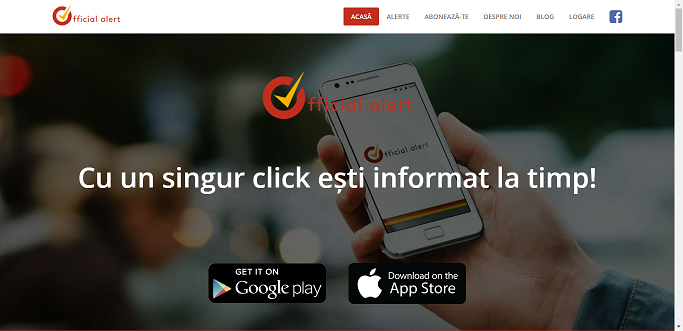
\includegraphics{header.png}\\
 
 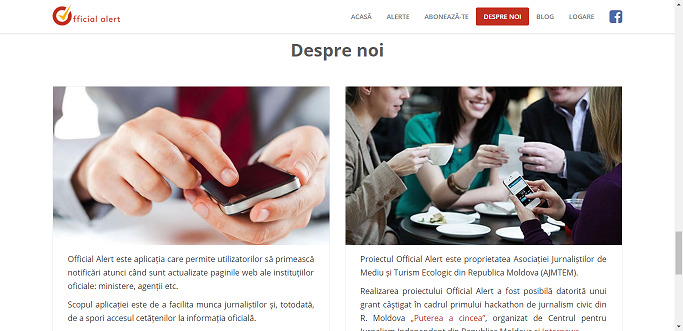
\includegraphics{about.png}\\
 
 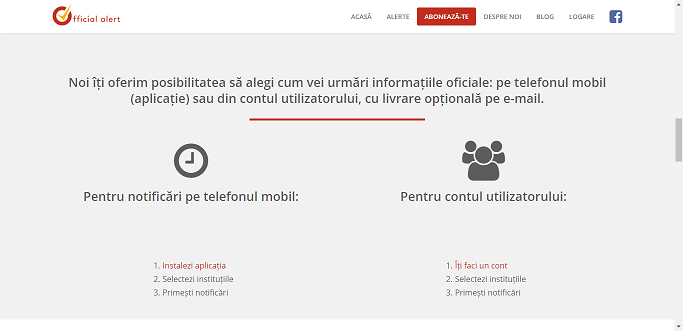
\includegraphics{aboneazate.png}\\ 
 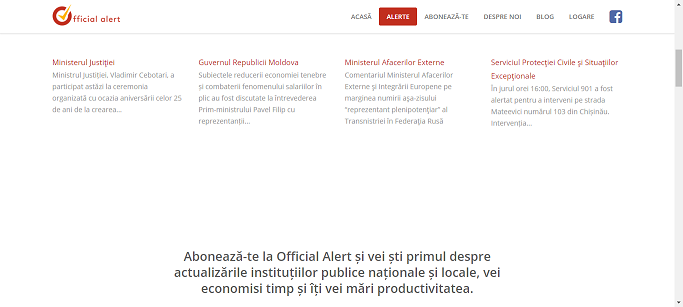
\includegraphics{alerte.png}\\
 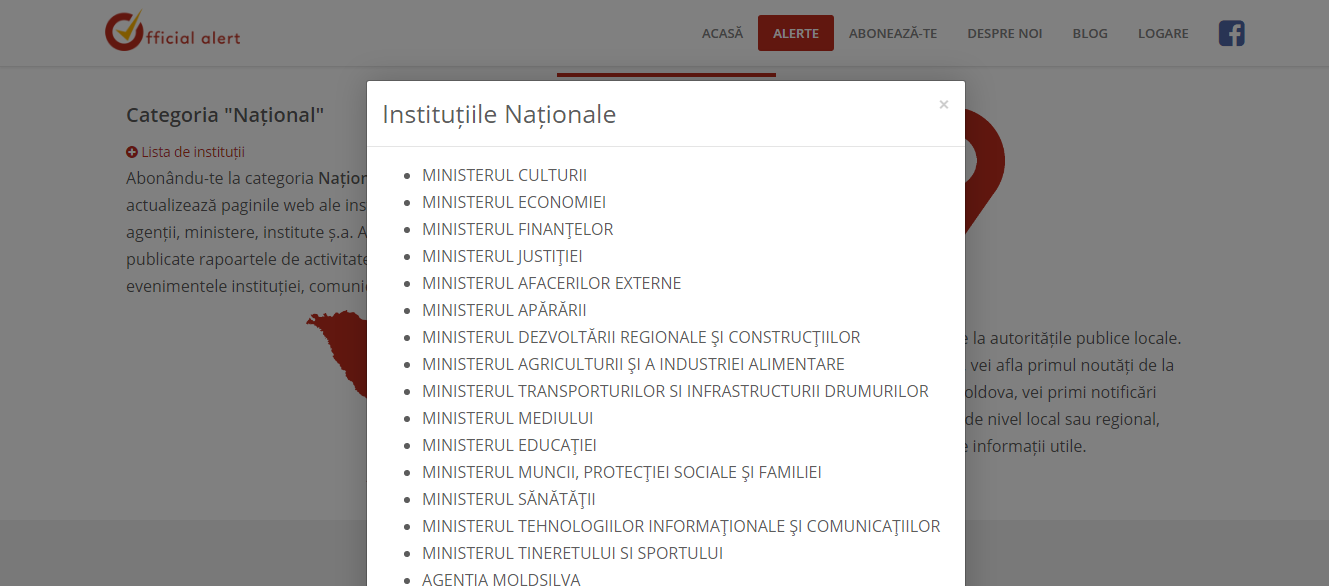
\includegraphics{popup.png}\\
 
 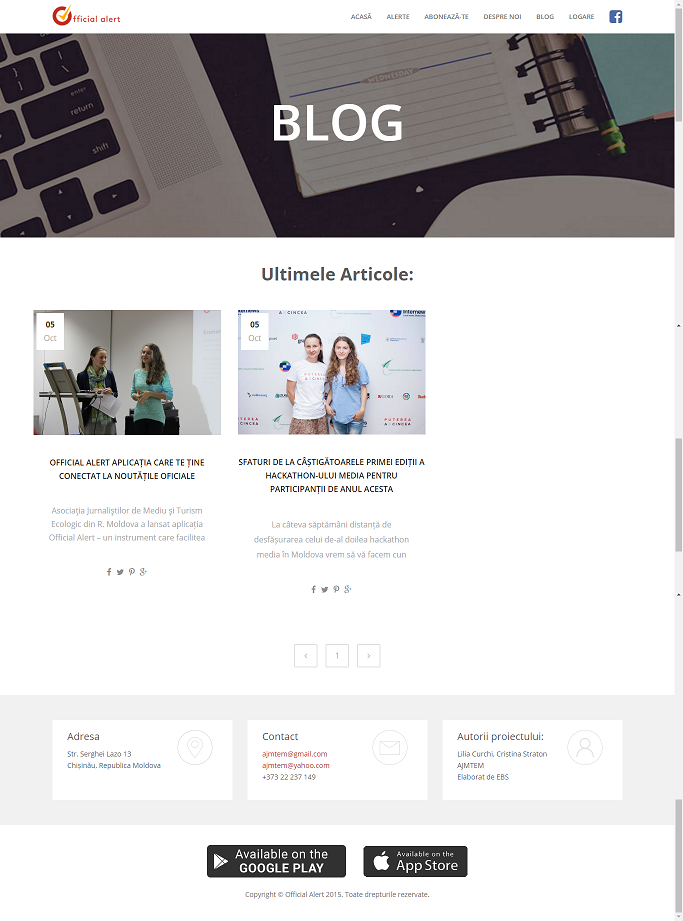
\includegraphics{page_blog.png}\\
 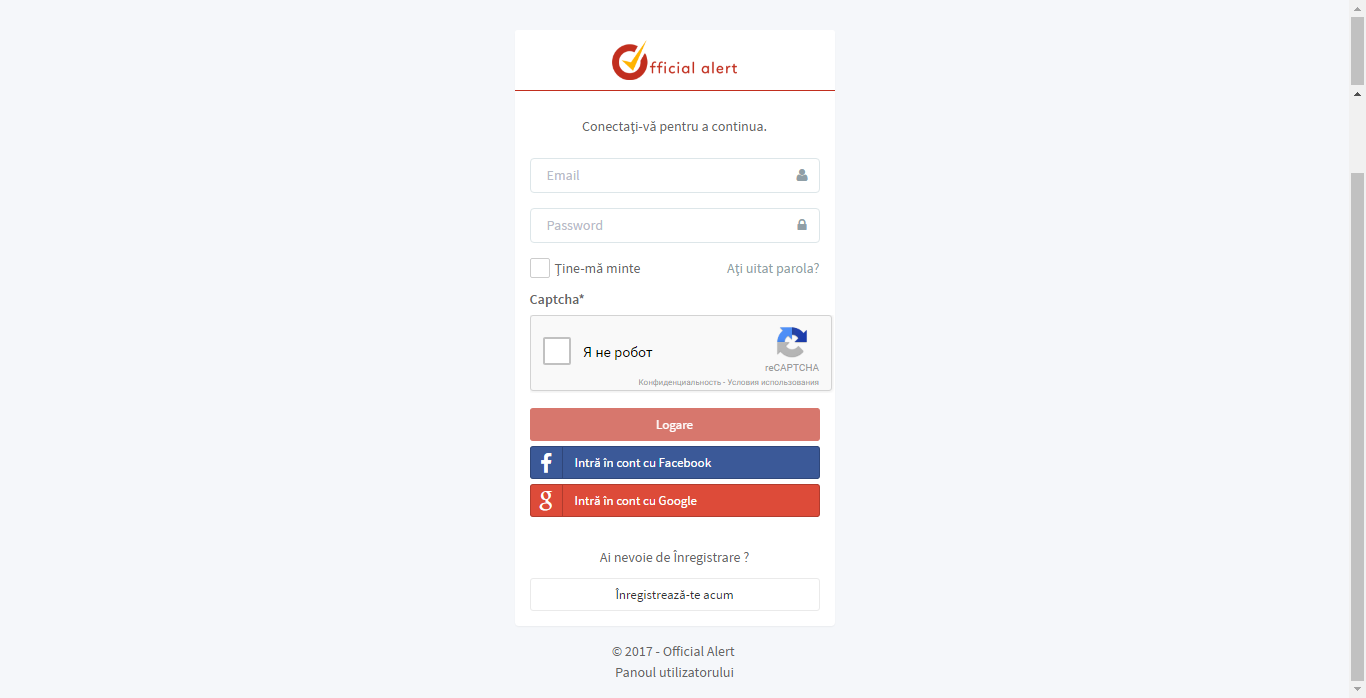
\includegraphics{log.png}\\
\section*{Concluzia}
Laboratorul dat am practicat structurarea  informaţiilor conţinutului paginilor web,deasemenea stilizare, modul şi locul în care sunt redate elementele HTML în pagină.
\end{document}